\documentclass[12pt,twoside,english,hyphens]{article}
\usepackage{charter}
\usepackage{helvet}
\usepackage[scaled=0.9]{beramono}
\usepackage[T1]{fontenc}
\usepackage[a4paper]{geometry}
\geometry{verbose,tmargin=2cm,bmargin=2cm,lmargin=2cm,rmargin=2cm}
\usepackage{fancyhdr}
\pagestyle{fancy}
\setcounter{tocdepth}{2}
\usepackage{babel}
\usepackage{array}
\usepackage{varioref}
\usepackage{float}
\usepackage{url}
\usepackage{amstext}
\usepackage{graphicx}
\usepackage{setspace}
\usepackage{longtable}
\onehalfspacing
\usepackage[unicode=true,
 bookmarks=true,bookmarksnumbered=true,bookmarksopen=false,
 breaklinks=false,pdfborder={0 0 0},backref=false,colorlinks=false]
 {hyperref}
\hypersetup{pdftitle={Design \& Code Group Project --- Report},
 pdfauthor={Dodd, Hill, Macrae, Oswald, Reily, Roblin, Saulais, Truesdale and Wyllie}}
 
\makeatletter

\renewcommand{\sfdefault}{FranklinGothic}

\usepackage{tocloft}
\renewcommand{\cfttoctitlefont}{\normalfont\sffamily\bfseries\huge}
\setlength{\cftaftertoctitleskip}{1.0cm}
\renewcommand{\cftsecfont}{\normalfont\sffamily\bfseries\large}
\renewcommand{\cftsecpagefont}{\normalfont\sffamily\bfseries\large}
\renewcommand{\cftsubsecfont}{\normalfont\sffamily}
\renewcommand{\cftsubsecpagefont}{\normalfont\sffamily}

\renewcommand{\cftloftitlefont}{\normalfont\sffamily\bfseries\Large}
\renewcommand{\cftfigfont}{\normalfont\sffamily}
\renewcommand{\cftfigpagefont}{\normalfont\sffamily}
\renewcommand{\cftlottitlefont}{\normalfont\sffamily\bfseries\Large}
\renewcommand{\cfttabfont}{\normalfont\sffamily}
\renewcommand{\cfttabpagefont}{\normalfont\sffamily}

\usepackage{titlesec}
\titleformat{\section}{\normalfont\Large\bfseries\sffamily}{\thesection}{1em}{}
\titleformat{\subsection}{\normalfont\large\bfseries\sffamily}{\thesubsection}{1em}{}
\titleformat{\subsubsection}{\normalfont\bfseries\sffamily}{\thesubsubsection}{1em}{}
\titleformat*{\paragraph}{\normalfont\bfseries\sffamily}

\titlespacing*{\section} {0pt}{3.5ex plus 1ex minus .2ex}{2.3ex plus .2ex}
\titlespacing*{\subsection} {0pt}{1.0ex plus 1ex minus .2ex}{0.5ex plus .2ex}
\titlespacing*{\subsubsection}{0pt}{1.0ex plus 1ex minus .2ex}{0.0ex plus .2ex}

%% superscript for citations
\def\@cite#1#2{$^{\mbox{\scriptsize [#1\if@tempswa , #2\fi]}}$}

\usepackage{pdfpages}
\usepackage{color}
\usepackage{parskip}
\setlength{\parindent}{0pt}
\fancyhead{}
\fancyhead[OL,EL]{\sffamily \leftmark}
\fancyfoot{}
\fancyfoot[EL]{\sffamily Design \& Code Group Project --- Report}
\fancyfoot[OR]{\sffamily Dodd, Hill, Macrae, Oswald, Reily, Roblin, Saulais, Truesdale and Wyllie}
\fancyfoot[OL,ER]{\sffamily \thepage}
\renewcommand{\headrulewidth}{0.4pt}
\renewcommand{\footrulewidth}{0.4pt}

\newcommand\centerAlign[1]{%
  \raisebox{-\height}{#1}%
}
\newcommand\bottomAlign[1]{%
  \raisebox{-0.5\height}{#1}%
}

%% Initial page numbering
\pagenumbering{roman}

\newcommand{\sectiontitle}[0]{}
\newcommand{\subsectiontitle}[0]{}
\renewcommand{\sectionmark}[1]{
    \markboth{#1}{}
    \renewcommand{\sectiontitle}{#1}
}
\renewcommand{\subsectionmark}[1]{
    \renewcommand{\subsectiontitle}{#1}
}

\newcommand{\authortitle}[2]{#1\hfill{}\textmd{\textit{\textrm{\small #2}}}}
\newcommand{\authorheadertitle}[2]{#1\hfill{}#2}
\newcommand{\authortoctitle}[2]{#1\hspace*{0.5em}\textmd{\textit{\textrm{\small (#2)}}}}

\newcommand{\sectionauthor}[2]{
    \section[\authortoctitle{#1}{#2}]{#1}%{\authortitle{#1}{#2}}
    \markboth{\authorheadertitle{#1}{#2}}{}
}
\newcommand{\subsectionauthor}[2]{
    \subsection[\authortoctitle{#1}{#2}]{#1}%{\authortitle{#1}{#2}}
    \markboth{\authorheadertitle{\sectiontitle \ --- #1}{#2}}{}
}
\newcommand{\subsubsectionauthor}[2]{
    \subsubsection[#1]{#1}%{\authortitle{#1}{#2}}}
    \markboth{\authorheadertitle{\sectiontitle \ --- \subsectiontitle}{#2}}{}
}

\newcommand{\sectionauthornotoc}[2]{
    \section*{#1}
    \markboth{\authorheadertitle{#1}{#2}}{}
}
\newcommand{\subsectionauthornotoc}[2]{
    \addtocounter{subsection}{1}
    \subsection*{\authortitle{\thesubsection\hspace*{1em}#1}{#2}}
}
\newcommand{\subsectionspeaker}[2]{
    %\subsectionauthornotoc{#1}{External speaker: #2}
    \subsection[#1]{\authortitle{#1}{External speaker: #2}}
}
\newcommand{\meetinginfo}[1]{\textit{\footnotesize #1}{\footnotesize \par}}
\newcommand{\appendixauthor}[2]{
    \addtocounter{section}{1}
    \addcontentsline{toc}{section}{\Alph{section} \hspace{0.1mm} \authortoctitle{Appendix: #1}{#2}}
    \markboth{\authorheadertitle{Appendix: #1}{#2}}{}
}

\newcommand{\appendixsection}[1]{
    \addtocounter{section}{1}
    \addcontentsline{toc}{section}{\Alph{section} \hspace{0.1mm} Appendix: #1}
    \markboth{Appendix: #1}{}
}

% use TexGyre Schola for tables (clone of Century Schoolbook)
\newcommand{\tablefont}[1]{{\fontfamily{qcs} \selectfont #1}}

% numbered equations
\renewcommand\[{\begin{equation}}
\renewcommand\]{\end{equation}}

\newcommand{\tm}{\textsuperscript{TM}}

\@ifundefined{showcaptionsetup}{}{%
 \PassOptionsToPackage{caption=false}{subfig}}
\usepackage{subfig}
\makeatother

\begin{document}

\includepdf{FrontPage.pdf}

\tocloftpagestyle{fancy}

\tableofcontents{}

\listoffigures
\listoftables
\clearpage{}

\pagenumbering{arabic}

\section*{Introduction}
\addcontentsline{toc}{section}{Introduction}
\markboth{Introduction}{}


\clearpage{}
\sectionauthor{Specifications}{Lauren Hill \& John Truesdale}
\documentclass[a4paper,11pt]{article}
\begin{document}

\section{Specification}
This section will report on the overall specification for the application and detail the resources that brought about its construction from the initial client specification to the known background information and current technologies employed. 

\subsection{Initial Concept}
The task set to the development team was to design, implement and evaluate an application for use by both researchers and students within the Mathematical and Computer Science (MACS) department's learning zone that utilized the Microsoft Kinect.

\subsection{Background Information}
The learning zone was purpose built within the waiting area between three of the MACS department's lecture facilities, as a social area for recreational or study use by students. In addition it provided researchers space from which to promote their work and acted as a central zone of information for all involved. It features three open planned seating arrangements in addition to two more enclosed work spaces with three, large TV screens positioned about the adjacent walls, each with their own Kinect sensor. 

\begin{center}
\textit{Image - Crush Area}
\end{center}

\subsection{Current Technologies}
Prior to the start of the project, the learning zone screens each featured an independent applications for displaying various information on content relevant to the department's subject area which ranged from displaying student and researcher work going on in the department, to twitter feeds highlighting headlines on topics of interest.

\subsection{Proposed Solution} 
A solution was proposed which involved displaying these various forms of content in a more central and uniform manner, in addition to serving as an interactive and social application that kept with the recreational aspect of the learning zone. This application would provide a premise from which to view the data but also a way in which users could interact with each other through the use of separate screens.

\section{Project Structure}
This section will detail the project structure employed in order to construct the application, from the modified methodology used to the projected schedule and utilized technologies.

\subsection{Methodology}
Due to the size of the group for the task at hand, it was decided that a SCRUM methodology modified with group micromanagement would be used. The group was split between two camps - three worked on the design, research and evaluation of the project, and six worked on the programming itself. At the top of each group was one individual responsible for managing their group's workload for the week to ensure deliverables were met, and finally collaborating everything at the end of the week into a format that was presentable to the client. As much as possible, this workload was split between smaller teams that were independent and relied as little as possible on each other in order to minimize the possibility of a domino effect in missing project deadlines.

\begin{center}
\textit{Image - Group Management Table}
\end{center}

\subsection{Timetable}
A routine schedule was decided for each week in order to facilitate regular meetings with the client and ensure the application's constant progression in the right direction. Each week a prototype was presented in a meeting with the client, where feedback was then received and a deliverable was decided for the week after. The group then met separately at least once a week to discuss how to achieve each deliverable with appropriate deadlines for each team, group and on an individual basis. A white board was used to document these tasks, as each member had easy access to it, and was referred to the week after for assessment of the group's progress. If needed, the group met again prior to the client's meeting or members of smaller teams met separately as needed to produce deliverables.

\subsection{Technology Utilized}
To keep the group in good contact with each other, BaseCamp was used as an online collaborative tool where announcements were made, milestones were set and each meeting's minutes were posted. This was to ensure that each member had the adequate resources and information in order to work towards their own personal deliverables. In addition GitHub was used as online source control in and was maintained solely by the code group leader.

\subsection{Project Schedule}
At the start of the project, a rough outline of all high level project deliverables was laid out within the twelve week timespan. This rough draft provided the project lead with a way of correlating at which point the group was in at any given time and thus determining if the project was on track. As an agile method was used to construct the application, each week the plan was updated, for better or for worse, and was modified to meet the client's weekly deliverables. The modified draft is detailed below:

\begin{description}
	\item[Week 1] - Client Specification
	\item[Week 2] - Initial Concept
	\item[Week 3] - Paper Prototype
	\item[Week 4] - Application Iteration \textit{(2)}
	\item[Week 5] - Client Evaluation
	\item[Week 6] - Application Iteration \textit{(3)} \textbf{*}
	\item[Week 7] - Client Evaluation
	\item[Week 8] - Application Iteration \textit{(4)} and User Evaluation
	\item[Week 9] - Evaluation and Application Iteration \textit{(5)} \textbf{*}
	\item[Week 10] - Draft Report and User Evaluation
	\item[Week 11] - Report Revision, Evaluation and Application Iteration \textit{(6)}
	\item[Week 12] - Final Report
\end{itemize}

\textbf{*} - A number of contingency weeks were placed within the initial timetable for additional development if required. If the contingency week was not needed, the objective was to produce further functionality and provide another iteration.

\section{Design}
In this section the overall design of the application will be detailed, specifically in regards to the initial requirements specification. In addition more detail will be discussed on the desired functionality for all aspects of the application from which a paper prototype will be constructed and evaluated as a goal for the final submission.

\subsection{Initial Concept}
The initial concept for the project was to construct an application that utilized the multiple, accessible screens in the learning zone. Each screen would display balloons which could ``float'' between them in a circular fashion. In addition, users would be able to interact with one or more balloons by waving their hands in a manner to ``push'' the balloons a certain way. There would be various types of balloons, from those displaying content from twitter feeds or user uploaded content, to simple ``customizable'' balloons that had no content.

Each balloon could be dropped into one of several paint buckets along the bottom of the screen in order to ``paint'' them a certain colour or pattern, and content balloons could be burst to reveal the full content inside. When burst, content would be displayed on a window in front of the screen for some time before disappearing on its own or being closed by the user. The content itself would be updated regularly as users uploaded their own content or the twitter feed updates, from which a particular number of each kind of balloon would be maintained at all times. In terms of the content, it would be either a series of twitter feeds which could provide the user with useful information or a custom content balloon which displayed desired text and graphic, all chosen by a user. A QR code would be provided for all balloons in order to allow the user to access the original source through the use of a QR Code reader on a smartphone. A later iteration brought forward the use of a rating system which would allow users to rate user content balloons which would then be affect their priority level and frequency on the screen.

Lastly, the application would incorporate a web client for users to submit their own content to be displayed on the screens on a balloon. It would allow users to enter in their desired text, provide a picture and web link, and customize their balloon's colour. In addition, their would be a moderator interface implemented within that would allow chosen users to delete any inappropriate content as filters were not to be considered as requested by the client.

\begin{center}
\textit{Please note that additional features were implemented over the course of the project but will not be detailed until later in the evaluation section of the report. This is because all extra requirements were constructed from user feedback.}
\end{center}

\subsection{Desired Functionality}
As the balloons are the main focus of the application, the abstract functionality will be considered as such; balloons must be created, displayed, and destroyed. In terms of creation, this will come about through the periodic updates of the twitter system and user content system. After being displayed on a random screen, the balloons must have the ability to transition onto another screen if one should reach the edge of its current screen. Finally, destruction of a balloon will occur when a user ``pops'' it or when the next patch of updates comes through; which will destroy all the current balloons. A maximum number of seven balloons will be loaded onto each screen, totaling twenty one balloons in total for three screens.

Each balloon had to serve two functions: being customizable and being interactive (the ability to be moved and burst). Customizing a balloon would happen by pushing it into a paint bucket, and depending on the kind of paint bucket involved, would react appropriately. There would be three buckets for each primary colour, allowing balloons to be dipped into multiple buckets and be blended (for example dipping a balloon into a red bucket and then a blue bucket would result in a purple balloon). In addition two pattern paint buckets (strips and spots) would exist and would provide an overlay to the balloon. Patterns would have a toggle setting, meaning the user could have no pattern by hitting the same bucket again.

Secondly, balloons would burst to reveal a more detailed view of their content. This view would appear like a secondary window over the main screen (but not taking up a high percentage of the available screen such that the background could not be seen) and after 30 seconds would disappear on its own. Optionally, a user may close the box early through the use of a red ``X'' in the corner of the screen. These content boxes would display their summary text along the top, their full text in the middle, and an image and QR code representing a URL to the original source. In the case of twitter content, the full text would be the entire tweet, the image would be the twitter account's user profile and the URL would simply link to the tweet itself. In the case of custom user content, the text, image and URL would all be as specified by the user through a separate web interface. Finally the screens needed to be able to communicate with each other to allow balloons to ``pass through'' with the appropriate information.

With regards to the rating system, the QR codes for custom user content would firstly redirect to an interim page on a user's phone that would allow the user to vote the content up or down (or not at all) before visiting the specified URL. This would then help better rated content appear more frequently over more badly rated content.

In terms of the web application, a user would be able to login with their MACS user name and password. All current user content would be displayed in a list format from which the user could access the information independently. In addition, a user would then be able to create their own content, which would then be added to the custom content system for possible selection. The administrative side of the application would only require the list of content with an additional delete option.

\subsubsection{Kinect}
In order to utilize the playful nature of the Kinect, and to encourage new users to pick up the concepts quickly, interaction with the application needed to be achieved in the most intuitive and simple way possible. The solution to this was to make the balloons physical entities that users are able to hit and push as desired. This one concept facilitates all functions - users customize balloons by pushing them into paint buckets, and burst balloons by squeezing them between their hands. The one exception to this is the close button on the content window, which is activated by a user hovering their hand over the button for a small length of time - a gesture which is frequently used in native Microsoft Kinect applications for menu selection.

\subsubsection{Twitter}
Content would be received from the university's Twitter account to ensure content that is relevant to the users of the learning zone is displayed. This would not be filtered and would be selected for display based on age where the newest content comes first.

\subsubsection{User Uploads}
Users would be able to upload their own custom content to be displayed as a balloon. Using an additional interface accessed through a web page a user would be able to define summary text to be displayed on the small boxes carried by the balloons, full text as displayed on the content window, an image to be displayed on the content window, a URL that the QR code will allow smartphone users to visit and the colour and pattern of their specific balloon. Using this, a user would be able to see their personal balloon on the screen displaying their student or research work as the original applications in the learning zone had fascilitated.

\subsection{Presentation}
With the application utilizing the Kinect and exhibiting a playful nature, a cartoon-like style was chosen to encourage play from its users. Bold primary colours and a simple art style were chosen in order to maintain the light-hearted feel of the learning zone as well as provide something pleasing to the eye when not in use. Balloons blown by a gentle breeze in addition to a bright blue sky with fluffy clouds were chosen to promote a relaxing atmosphere, in addition to comical paint buckets.

Design patterns were referenced for the layout of the interface, keeping all customization tools along the bottom of the screen and fully maximizing screen space for the balloons by partially hiding the paint buckets when no balloons are nearby. 

\subsection{Scope, Limitations and Assumptions}
As no preliminary research was conducted before the start of the design, but was carried out during it, accessibility was not considered for the application. A number of Kinect limitations were discovered but as these were a hardware disability, they are located under the appropriate heading for future evaluation. In addition, sound and visual cues were not implemented but were investigated and will also be included within the future work section of the report.

\subsection{Paper Prototype}
A paper prototype was constructed to demonstrate one screen of the application's design to the client. It showed user interactivity, in relation to balloon customization, including the movement of the paint buckets and the bursting of balloons to reveal content. In addition it demonstrated two different approaches to displaying balloons - on their own or as carrying boxes with summary text for each piece of content - the latter of which was chosen by the client. The paper prototype received positive feedback and incorporated all desired functionality and thus was the basis for the software design that was to follow.

\begin{center}
\textit{Image - Paper Prototype}
\end{center}

\end{document}

\clearpage{}
\sectionauthor{Research}{Ryan Oswald}
%\input{Research.tex}

\clearpage{}
\sectionauthor{Project Structure}{Lauren Hill \& John Truesdale}
This section will detail the project structure employed in order to construct the application, from the modified methodology used to the projected schedule and utilized technologies.

\subsection{Methodology}
Due to the size of the group for the task at hand, it was decided that a SCRUM methodology modified with group micromanagement would be used. The group was split between two camps - three worked on the design, research and evaluation of the project, and six worked on the programming itself. At the top of each group was one individual responsible for managing their group's workload for the week to ensure deliverables were met, and finally collaborating everything at the end of the week into a format that was presentable to the client. As much as possible, this workload was split between smaller teams that were independent and relied as little as possible on each other in order to minimize the possibility of a domino effect in missing project deadlines.

\begin{center}
\textit{Image - Group Management Table}
\end{center}

\subsection{Timetable}
A routine schedule was decided for each week in order to facilitate regular meetings with the client and ensure the application's constant progression in the right direction. Each week a prototype was presented in a meeting with the client, where feedback was then received and a deliverable was decided for the week after. The group then met separately at least once a week to discuss how to achieve each deliverable with appropriate deadlines for each team, group and on an individual basis. A white board was used to document these tasks, as each member had easy access to it, and was referred to the week after for assessment of the group's progress. If needed, the group met again prior to the client's meeting or members of smaller teams met separately as needed to produce deliverables.

\subsection{Technology Utilized}
To keep the group in good contact with each other, BaseCamp was used as an online collaborative tool where announcements were made, milestones were set and each meeting's minutes were posted. This was to ensure that each member had the adequate resources and information in order to work towards their own personal deliverables. In addition GitHub was used as online source control in and was maintained solely by the code group leader.

\subsection{Project Schedule}
At the start of the project, a rough outline of all high level project deliverables was laid out within the twelve week timespan. This rough draft provided the project lead with a way of correlating at which point the group was in at any given time and thus determining if the project was on track. As an agile method was used to construct the application, each week the plan was updated, for better or for worse, and was modified to meet the client's weekly deliverables. The modified draft is detailed below:

\begin{description}
	\item[Week 1] - Client Specification
	\item[Week 2] - Initial Concept
	\item[Week 3] - Paper Prototype
	\item[Week 4] - Application Iteration \textit{(2)}
	\item[Week 5] - Client Evaluation
	\item[Week 6] - Application Iteration \textit{(3)} \textbf{*}
	\item[Week 7] - Client Evaluation
	\item[Week 8] - Application Iteration \textit{(4)} and User Evaluation
	\item[Week 9] - Evaluation and Application Iteration \textit{(5)} \textbf{*}
	\item[Week 10] - Draft Report and User Evaluation
	\item[Week 11] - Report Revision, Evaluation and Application Iteration \textit{(6)}
	\item[Week 12] - Final Report
\end{description}

\textbf{*} - A number of contingency weeks were placed within the initial timetable for additional development if required. If the contingency week was not needed, the objective was to produce further functionality and provide another iteration.


\clearpage{}
\sectionauthor{Design}{Lauren Hill \& John Truesdale}
In this section the overall design of the application will be detailed, specifically in regards to the initial requirements specification. In addition more detail will be discussed on the desired functionality for all aspects of the application from which a paper prototype will be constructed and evaluated as a goal for the final submission.

\subsection{Initial Concept}
The initial concept for the project was to construct an application that utilized the multiple, accessible screens in the learning zone. Each screen would display balloons which could ``float'' between them in a circular fashion. In addition, users would be able to interact with one or more balloons by waving their hands in a manner to ``push'' the balloons a certain way. There would be various types of balloons, from those displaying content from twitter feeds or user uploaded content, to simple ``customizable'' balloons that had no content.

Each balloon could be dropped into one of several paint buckets along the bottom of the screen in order to ``paint'' them a certain colour or pattern, and content balloons could be burst to reveal the full content inside. When burst, content would be displayed on a window in front of the screen for some time before disappearing on its own or being closed by the user. The content itself would be updated regularly as users uploaded their own content or the twitter feed updates, from which a particular number of each kind of balloon would be maintained at all times. In terms of the content, it would be either a series of twitter feeds which could provide the user with useful information or a custom content balloon which displayed desired text and graphic, all chosen by a user. A QR code would be provided for all balloons in order to allow the user to access the original source through the use of a QR Code reader on a smartphone. A later iteration brought forward the use of a rating system which would allow users to rate user content balloons which would then be affect their priority level and frequency on the screen.

Lastly, the application would incorporate a web client for users to submit their own content to be displayed on the screens on a balloon. It would allow users to enter in their desired text, provide a picture and web link, and customize their balloon's colour. In addition, their would be a moderator interface implemented within that would allow chosen users to delete any inappropriate content as filters were not to be considered as requested by the client.

\begin{center}
\textit{Please note that additional features were implemented over the course of the project but will not be detailed until later in the evaluation section of the report. This is because all extra requirements were constructed from user feedback.}
\end{center}

\subsection{Desired Functionality}
As the balloons are the main focus of the application, the abstract functionality will be considered as such; balloons must be created, displayed, and destroyed. In terms of creation, this will come about through the periodic updates of the twitter system and user content system. After being displayed on a random screen, the balloons must have the ability to transition onto another screen if one should reach the edge of its current screen. Finally, destruction of a balloon will occur when a user ``pops'' it or when the next patch of updates comes through; which will destroy all the current balloons. A maximum number of seven balloons will be loaded onto each screen, totaling twenty one balloons in total for three screens.

Each balloon had to serve two functions: being customizable and being interactive (the ability to be moved and burst). Customizing a balloon would happen by pushing it into a paint bucket, and depending on the kind of paint bucket involved, would react appropriately. There would be three buckets for each primary colour, allowing balloons to be dipped into multiple buckets and be blended (for example dipping a balloon into a red bucket and then a blue bucket would result in a purple balloon). In addition two pattern paint buckets (strips and spots) would exist and would provide an overlay to the balloon. Patterns would have a toggle setting, meaning the user could have no pattern by hitting the same bucket again.

Secondly, balloons would burst to reveal a more detailed view of their content. This view would appear like a secondary window over the main screen (but not taking up a high percentage of the available screen such that the background could not be seen) and after 30 seconds would disappear on its own. Optionally, a user may close the box early through the use of a red ``X'' in the corner of the screen. These content boxes would display their summary text along the top, their full text in the middle, and an image and QR code representing a URL to the original source. In the case of twitter content, the full text would be the entire tweet, the image would be the twitter account's user profile and the URL would simply link to the tweet itself. In the case of custom user content, the text, image and URL would all be as specified by the user through a separate web interface. Finally the screens needed to be able to communicate with each other to allow balloons to ``pass through'' with the appropriate information.

With regards to the rating system, the QR codes for custom user content would firstly redirect to an interim page on a user's phone that would allow the user to vote the content up or down (or not at all) before visiting the specified URL. This would then help better rated content appear more frequently over more badly rated content.

In terms of the web application, a user would be able to login with their MACS user name and password. All current user content would be displayed in a list format from which the user could access the information independently. In addition, a user would then be able to create their own content, which would then be added to the custom content system for possible selection. The administrative side of the application would only require the list of content with an additional delete option.

\subsection{Kinect}
In order to utilize the playful nature of the Kinect, and to encourage new users to pick up the concepts quickly, interaction with the application needed to be achieved in the most intuitive and simple way possible. The solution to this was to make the balloons physical entities that users are able to hit and push as desired. This one concept facilitates all functions - users customize balloons by pushing them into paint buckets, and burst balloons by squeezing them between their hands. The one exception to this is the close button on the content window, which is activated by a user hovering their hand over the button for a small length of time - a gesture which is frequently used in native Microsoft Kinect applications for menu selection.

\subsection{Twitter}
Content would be received from the university's Twitter account to ensure content that is relevant to the users of the learning zone is displayed. This would not be filtered and would be selected for display based on age where the newest content comes first.

\subsection{User Uploads}
Users would be able to upload their own custom content to be displayed as a balloon. Using an additional interface accessed through a web page a user would be able to define summary text to be displayed on the small boxes carried by the balloons, full text as displayed on the content window, an image to be displayed on the content window, a URL that the QR code will allow smartphone users to visit and the colour and pattern of their specific balloon. Using this, a user would be able to see their personal balloon on the screen displaying their student or research work as the original applications in the learning zone had facilitated.

\subsection{Presentation}
With the application utilizing the Kinect and exhibiting a playful nature, a cartoon-like style was chosen to encourage play from its users. Bold primary colours and a simple art style were chosen in order to maintain the light-hearted feel of the learning zone as well as provide something pleasing to the eye when not in use. Balloons blown by a gentle breeze in addition to a bright blue sky with fluffy clouds were chosen to promote a relaxing atmosphere, in addition to comical paint buckets.

Design patterns were referenced for the layout of the interface, keeping all customization tools along the bottom of the screen and fully maximizing screen space for the balloons by partially hiding the paint buckets when no balloons are nearby. 

\subsection{Scope, Limitations and Assumptions}
As no preliminary research was conducted before the start of the design, but was carried out during it, accessibility was not considered for the application. A number of Kinect limitations were discovered but as these were a hardware disability, they are located under the appropriate heading for future evaluation. In addition, sound and visual cues were not implemented but were investigated and will also be included within the future work section of the report.

\subsection{Paper Prototype}
A paper prototype was constructed to demonstrate one screen of the application's design to the client. It showed user interactivity, in relation to balloon customization, including the movement of the paint buckets and the bursting of balloons to reveal content. In addition it demonstrated two different approaches to displaying balloons - on their own or as carrying boxes with summary text for each piece of content - the latter of which was chosen by the client. The paper prototype received positive feedback and incorporated all desired functionality and thus was the basis for the software design that was to follow.

\begin{center}
\textit{Image - Paper Prototype}
\end{center}


\clearpage{}
\sectionauthor{System Architecture}{Andrew Dodd}
%\documentclass{article}
%\usepackage{graphicx}

%\title{Balloons Project - System Architecture}
%\author{Andrew Dodd}
%\begin{document}
%\maketitle

\subsection{Introduction}
This document gives an overview of the entire Balloons Project system along 
with a brief description of its main components. Further details on each 
individual system can be found in the corresponding section of documentation.

\subsection{System Overview}

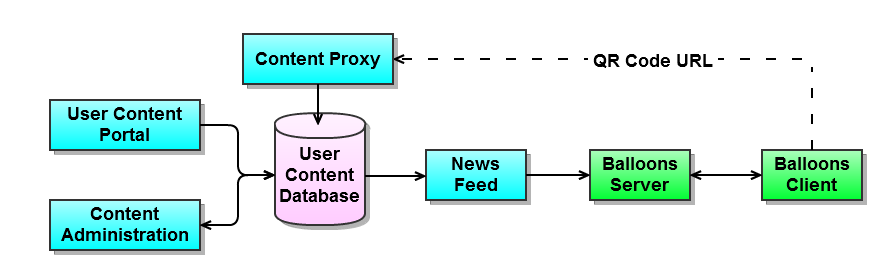
\includegraphics[width=\textwidth]{Diagrams/System-Architecture-Diagram.png}

Items in light blue are web-based components, written in PHP and producing 
either HTML/JS/CSS page output or JSON objects. Green items are written in C\#
4.0 and the pink database is an SQL RDBMS. The QR Code URL is accessed by users
when viewing content and is usually interpreted by a third-party device such as
a mobile phone.

\subsubsection{User Content Database}
The User Content Database is used to store user content submitted from the web
front end. Important information stored includes general content information 
such as title and image; when the content was submitted; and the name of the 
user who submitted the content (for moderation purposes and deter the 
submission of inappropriate content). The database also stores the current 
"score" of each custom article; this comes from the content voting system. 

\subsubsection{Web-Front Ends: User Content Portal \& Content Administration}
Two web-based front ends exist. The User Content Portal is used by users to 
submit custom content which will appear as a balloon on the system. Once 
content is submitted it is stored in the User Content Database. The Content
Administration section lets administrators review and moderate any user 
generated content and will be primarily used to remove offensive or otherwise
inappropriate content.

\subsubsection{Content Proxy}
The content proxy is used to provide an interface for end users to rate content
by either giving it an up or down vote. Once the vote is cast, it is stored
against the story in the database and the user is redirected to the URL of the
content.

\subsubsection{News Feed}
The News Feed component is responsible for choosing some content for the 
front-end; ratios for the different content-types are defined in the feed 
whilst the number of items to fetch is determined by the caller. When 
requested, it generates a JSON object which is consumed by the Balloons Server.

\subsubsection{Balloon Server}
The Balloon Server is responsible for coordinating all the balloons on the 
Balloon Clients. This involves parsing the News Feed to get balloons, sending
balloons to each client and dealing with balloons travelling between screens 
as well as balloons being popped by the user. 

When a client connects to the server, it must generate new balloons; this 
causes the feed to be refreshed. Once the balloons are generated they are 
pushed to the new client. If a client disconnects, all its balloons are 
randomly redistributed to the other screens.

\subsubsection{Balloon Client}
The Balloon Client displays balloons in a graphical manner and allows users to
interact with the display. The main elements of the display are the balloons 
themselves which have a short description of the article they represent and the
news-reader element which displays the full content of the article as well as
an image and QR Code which directs users via the Content Proxy to the news item.

%\end{document}


\clearpage{}
\sectionauthor{Client Design}{Andrew Dodd}
This section describes the Balloons Client system in detail and gives
reasoning behind some of the design decisions that were made. The Client system
is the system which the user interacts with on the screen; it makes use of the
Microsoft Kinect hardware to provide natural user input and connects to the 
Balloons Server to manage the items on screen. 

This document only describes the technical aspects of the Client system; for 
design decisions and specification relating to the user interface and input 
controllers please consult the Client Design document.

\subsection{System Design}
As much as is possible, the Client system is split into four components: 
Network, Graphics, Physics and Input; however these four components also need 
to be tied up in a central location --- XNA puts the burden of this into the Game
class. With the exception of Graphics which is part of the Game class, each
sub-system has its own code package and is quite discrete from all the other 
parts, i.e. these components are loosely coupled.

The other main part of the Client system is the model objects --- these represent
some of the main objects in the game. They are not true model objects in the
MVC pattern --- some of the models actually contain drawing logic. This allows
the drawing methods to be moved out of the main graphics system and makes the
system more coherent.

\subsection{Models}
\subsubsection{Bucket}
The bucket model represents a paint bucket which can be used to change the 
decoration of a balloon. A bucket implementation should implement the abstract
Apply To Balloon method to perform the decoration. Two buckets are currently
included in the system: one which changes the colour of the balloon and one 
which changes the overlay. 

\subsubsection{Client Balloon}
The client balloon model represents a balloon as it appears on screen. It 
contains information pertaining to the balloon's dimensions and also a cache of
any textures which have been generated for that balloon (its image or QR code, 
for example). 

\subsubsection{Client Plane}
The client plane model represents a plane as it appears on the screen, as well
as the banner that it carries along with it.

\subsubsection{Content Box}
The content box model is used to define the logic for drawing a content box to
the screen. Two content box implementations are available: one which uses raw
XNA drawing calls to position elements, and one which uses HTML to render the
content. The HTML renderer was a feature added mid-way through development but
is now the default model as it is easier to customize and looks much more
appealing. 

\clearpage{}
\subsection{Network Subsystem}
The Network Subsystem implements the INetworkManager interface and is 
responsible for managing communication between the Client and Server. The 
default implementation relies on the ScreenConnection class from the Messaging
library, details of which can be found elsewhere. 

\begin{table}[H]
\begin{tabular}{|p{4.8cm}|p{3.8cm}|p{7cm}|}
\hline
\multicolumn{3}{|c|}{INetworkManager} \\ \hline
Connect & & Connects the Network Manager to the Server. \\ \hline

MoveBalloonOffscreen & Balloon,\newline Direction,\newline Exit Position,\newline Velocity &
Sends a message to the Server telling it the given balloon has moved off 
screen. The direction is the side the balloon exited, the position a number 
between 0 and 1 of the height of the balloon, and velocity the velocity of the
balloon as it left. \\ \hline

NotifyBalloonPopped & Balloon & 
Sends a message to the Server telling it the given balloon has been popped by
the user. \\ \hline

GetBalloonDetails & Balloon ID &
Retrieves the details of the given balloon from its ID. \\ \hline

UpdateBalloonDetails & Balloon & 
Processes messages from the Server and will be called once per Update loop.
The four parameters are Actions which are called when the relevant message is
received from the Server. \\ \hline

ProcessMessages & On New Balloon,\newline On Pop Balloon,
\newline On Content Update,\newline On State 
Update &
Processes messages from the Server and will be called once per Update loop. 
The four parameters are Actions which are called when the relevant message is
received from the Server. \\ \hline
\end{tabular}

\caption{\emph{INetworkManager} reference}

\label{NetworkManagerRef}
\end{table}

\clearpage{}
\subsection{Physics Subsystem}
The Physics Subsystem is concerned with tracking physical objects in the game
and generates events based on collisions between them. This subsystem is 
slightly more coupled than other classes as it is not coded to an interface; 
this is because the physics and graphics systems are quite interdependent. 
Several methods are available on the Physics Manager to translate from world 
co-ordinates to screen ones. 

During the main loop, the Game System has to feed in the co-ordinates from the
Input system to the Physics system in order for the positions of the hands to 
be updated correctly. The Physics Manager makes use of a class called World
Entity; this class represents an object as it is stored in the world and is 
used by the Game System to track the relationship between physical entities and
model objects.

\begin{longtable}{|p{4.5cm}|p{3.5cm}|p{7.7cm}|}
\caption{\emph{PhysicsManager} reference \label{PhysicsManagerRef}}
\\
\hline
\multicolumn{3}{|c|}{PhysicsManager} \\ \hline

Initialize & Hand Size &
Initialises the Physics Manager. In our system, this creates the Farseer World
object. The Hand Size is provided as it is based on the size of the texture 
loaded in. \\ \hline

Update & Game Time &
Advances the physics world by the specified time. This is called once per call
of the Update method in the Game System.\\ \hline

Create Balloon & Position,\newline Velocity,\newline \emph{Returns} World Entity &
Creates a World Entity object for a balloon. This object will be added to the 
Physics Manager's internal list of Balloons and will cause events to fire when
certain collisions are detected with it.\\ \hline

Create Boundary & Width,\newline Position,\newline \emph{Returns} World Entity &
Creates a physical boundary in the system --- used to create the roof and the 
floor. Currently only horizontal boundaries can be created by this function.
Vertical boundaries are not handled by the physics engine but by the Game (as 
they fire network events).\\ \hline

Update Hand Positions & Array of Hands &
Updates the positions of the hands in the system. If a Hand object passed in 
is not currently tracked by the system, a new World Entity is created for it.
\\ \hline

Get Hand Positions & \emph{Returns} List of World Entity &
Returns the World Entity object for each hand currently tracked by the system.
\\ \hline

Get Hand For Entity & World Entity,\newline \emph{Returns} Hand &
Returns the Hand object for the World Entity provided. Used by the Game System
to draw the hand on screen. \\ \hline

Enable Handle Collisions & &
Enables collisions between hands and balloons. \\ \hline

Disable Hand Collisions & &
Disables collisions between hands and balloons. Used when the content box is 
up to avoid the weird feeling of colliding with balloons that the user can't 
see. \\ \hline

Apply Wind & & 
Applies a force to all the balloons to simulate wind. \\ \hline

Remove Entity & World Entity &
Removes the given entity from the physics world. Hand entities are not removed
with this function and would be regenerated on the next call to Update Hand 
Positions anyway. \\ \hline

\emph{Static} World To Pixel & World Position\newline \emph{Returns} Screen Position &
Converts a physics world co-ordinate to a screen co-ordinate.\\ \hline

\emph{Static} Pixel To World & Screen Position\newline \emph{Returns} World Position &
Converts a screen co-ordinate to a physics world one.\\ \hline

\emph{Static} World Body To Pixel & World Position,\newline Pixel Offset,\newline 
\emph{Returns} Screen Position &
Converts a physics world co-ordinate to a screen co-ordinate, minus a pixel 
offset (usually the width of a texture).\\ \hline

\emph{Static} Pixel To World Body & Screen Position,\newline Pixel Offset,\newline
\emph{Returns} World Position & 
As World Body to Pixel but in reverse.\\ \hline

\emph{Event} Balloon Popped & BalloonPopped\-EventArgs &
Fired when the Physics Manager detects that a user has popped a balloon.
\\ \hline

\emph{Event} Bucket Collision & BucketCollision\-EventArgs & 
Fired when the Physics Manager detects that a balloon has collided with a 
bucket.\\ \hline

\end{longtable}

\clearpage{}
\subsection{Input Subsystem}
The Input Subsystem tracks user input and is defined by the IInputManager
interface (see table \ref{InputManagerRef}. Two input subsystems are implemented in 
the project: one for using the Kinect, and one for using the Mouse. The Kinect 
system is described elsewhere in this report; the Mouse system is very simple in 
comparison.
 
When no mouse buttons are pressed, the mouse emulates a single hand which is
centred on the position of the mouse. If the left mouse button is held down, a
second hand appears with its position relative to the first hand. If, whilst
still the left mouse button is still down, the right mouse button is also
depressed, then the two hands will emulate a clapping motion.

\begin{table}[H]
\begin{tabular}{|p{3.6cm}|p{3cm}|p{9cm}|}
\hline
\multicolumn{3}{|c|}{IInputManager} \\ \hline
Initialize & Screen Size & 
Initialises the Input Manager. Some Input Devices use normalised dimensions so
the screen size parameter should be stored as the values returned by this 
Interface should be in screen co-ordinates. \\ \hline

GetHandPositions & \emph{Returns} Hand[] &
Returns an array of Hand objects, one Hand per physical hand. A Hand object
describes the position of a single hand and has an identifier to tell which
user the hand belongs to. 
The Hand objects must be static between calls; i.e. a Hand object should
represent a physical hand for the duration of said hand being focused as an
input entity. If this is not the case, and a new Hand object is generated 
every frame, the physics engine will not work correctly. \\ \hline
\end{tabular}
\caption{\emph{IInputManager} reference}

\label{InputManagerRef}
\end{table}

\subsection{Graphics \& Game Systems}
The main logic for the Graphics Subsystem lies in the Game System itself. XNA
defines a layout for the Game System, in which game logic should be performed
in the Update method and drawing logic in the Draw method (see table
\vref{BalloonClientRef}). The Game System also
ties together all the other components.

\begin{table}
\begin{tabular}{|p{3cm}|p{3.6cm}|p{9cm}|}
\hline
\multicolumn{3}{|c|}{BalloonClient} \\ \hline
\emph{Constructor} & Network Manager, Input Manager & 
Creates a new instance of the Balloon Client using the provided Network and 
Input Managers. (These are injected from the main method which determines which
to use from the Configuration object). This constructor also creates the 
Graphics Device Manager used by XNA and initialises the Input Manager with the
screen dimensions. \\ \hline

Load Content & & 
This is a method called by XNA and is used to load external content. It creates
a new Sprite Batch, loads in fonts and textures, and sets up the mappings so we
can access the textures quickly and easily in code. \\ \hline

Initialize & &
Initialize sets up the Physics Manager and the collision detection handlers, 
then creates the roof and floor boundaries. It creates the buckets using a 
formula to determine the gap between them. Finally, it asks the Network Manager
to connect to the server. \\ \hline

Update & Game Time &
Update performs the game logic. The following steps are performed:
\begin{itemize}
	\item{Process Network Events}
	\item{Process Input}
	\item{Process Physics (and Apply Wind)}
	\item{Move any balloons to other screens which have moved off the edge of the screen}
	\item{Update any running animations}
	\item{Update the content box (if it is visible)}
\end{itemize}
\\ \hline

Draw & Game Time &
Draw performs the actual drawing of the game world. It is not supposed to 
perform any logic tasks. Items drawn first will be hidden ``behind'' items drawn
later. The following steps are performed:
\begin{itemize}
	\item{Clear the screen and initialise the Sprite Batch}
	\item{Draw the background}
	\item{Draw the balloon captions}
	\item{Draw the balloons}
	\item{Draw the ``pop'' animations}
	\item{Draw the buckets}
	\item{Draw the content box (if it is supposed to be visible)}
	\item{Draw the user's hands}
	\item{Flush the Sprite Batch}
\end{itemize}
\\ \hline
\end{tabular}
\caption{\emph{BalloonClient} reference}

\label{BalloonClientRef}
\end{table}

\clearpage{}
\subsection{Development Report}
Throughout the development cycle of the project, several builds were presented
to the client. In the first few weeks, many of the demo builds were individual
feasibility studies of individual components needed to build the final project.
This section gives details of what requirements were implemented in the Client
system for each week.

\subsubsection{Client Demo 1 - 7th February}
\begin{figure}[h]
\begin{centering}
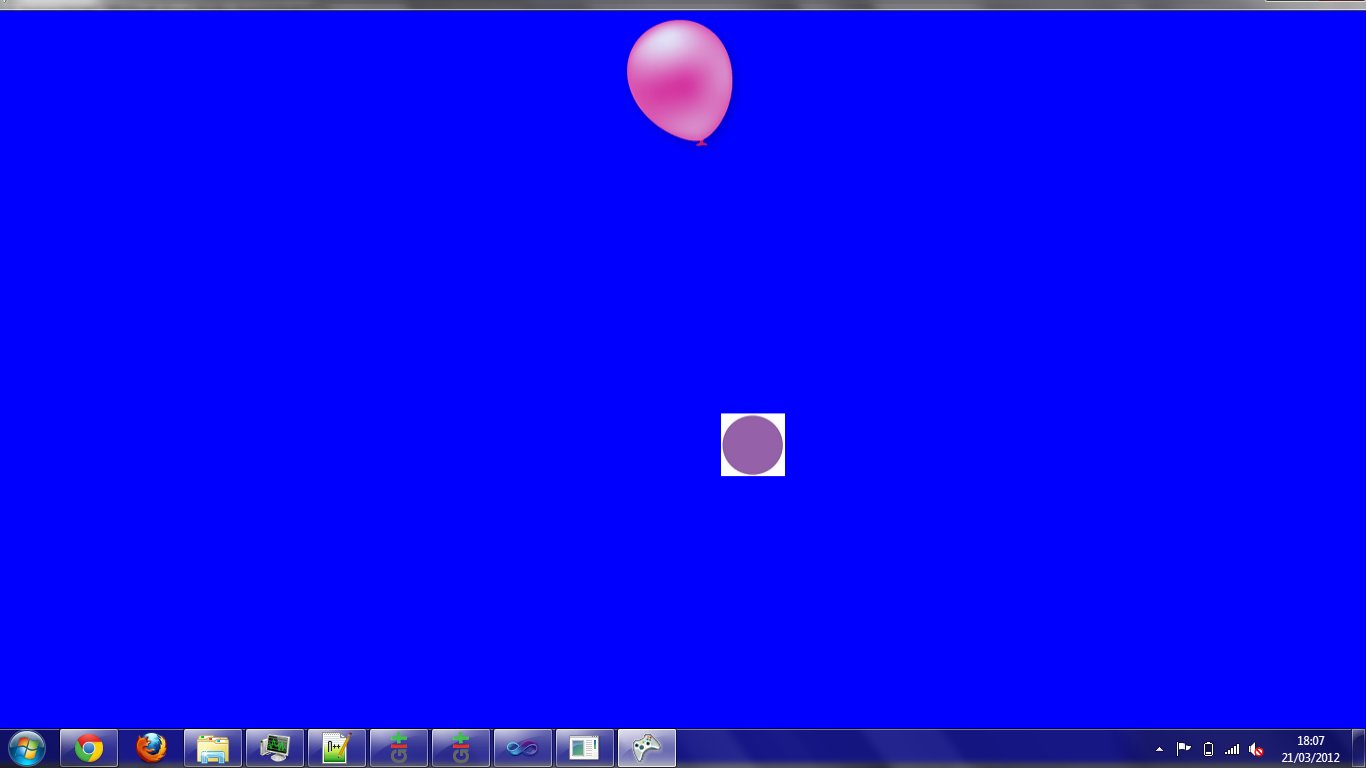
\includegraphics[width=\textwidth]{Diagrams/Client-Log-W4.jpg}
\par\end{centering}

\caption{Prototype in Week 4}
\end{figure}
The first prototype presented to the client showed hand tracking using the
Kinect and the capabilities of the physics engine using mock graphics. The
client thought that the Kinect input seemed to work well and was generally
pleased with the input at this stage.

Another prototype build during this week's meeting demonstrated the design of
the user interface which the user was also pleased with; however that prototype
was discarded as it was easier to implement the design on top of the input
prototype.

\subsubsection{Client Demo 2 - 14th February}
\begin{figure}[h]
\begin{centering}
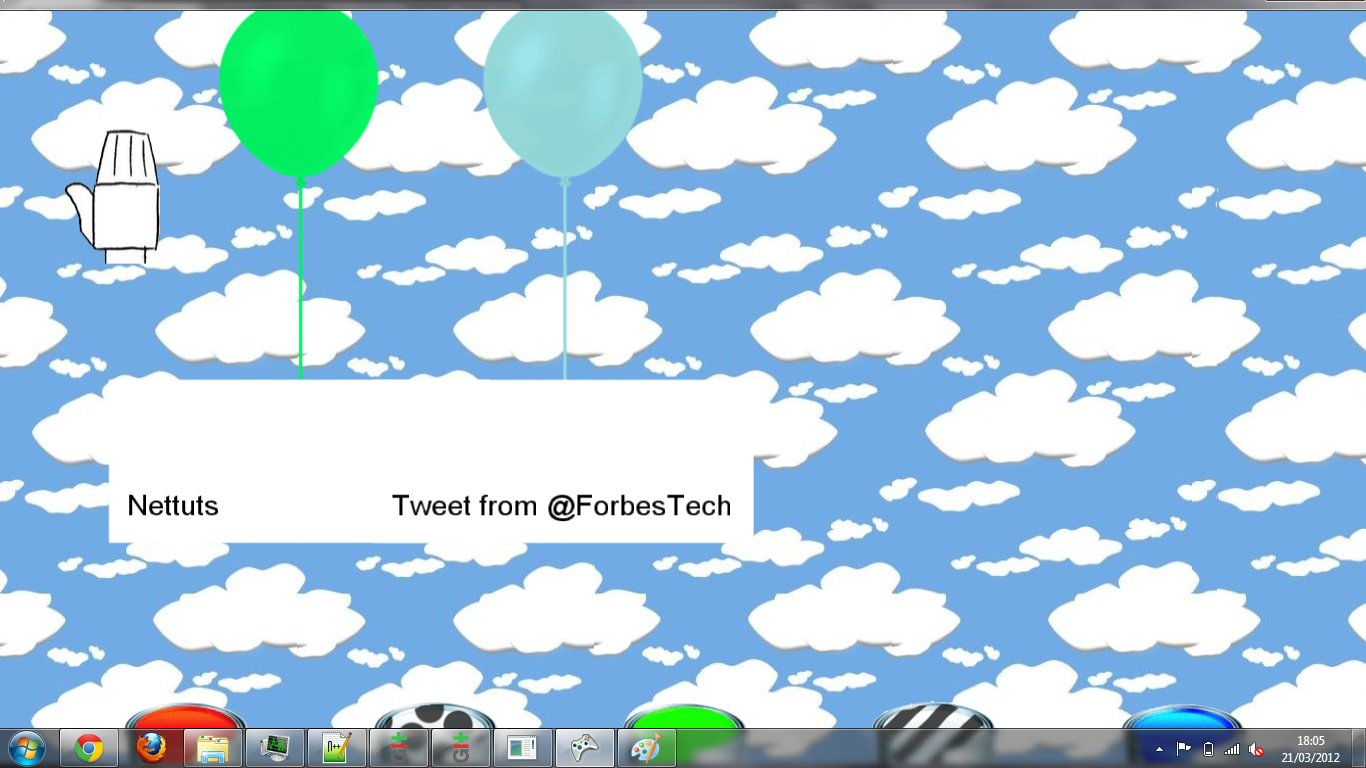
\includegraphics[width=\textwidth]{Diagrams/Client-Log-W5.jpg}
\par\end{centering}

\caption{Prototype in Week 5}
\end{figure}
The second demo prototype was much more advanced than the first. Many of the UI
concepts were implemented including balloons along with buckets to provide the 
``painting'' functionality. The mock graphics used in the first prototype were 
replaced by nicer images. The balloons were already tied into the physics 
however the rules were tweaked to make them much more realistic. The ability to
view the content of a balloon was also added by putting in a ``pop balloon'' 
action in the Input interface, which when called, caused a content box to open
with the desired content. Balloons were also given a small ``tag'' with a short
text description.

The Kinect input system was now governed by the physics engine. Whilst this 
allowed for collision detection, the user input lag added caused the client 
some issues as it ran very slowly on the target hardware. Furthermore, the
client had issues reaching the top of the screen on the target hardware.

Finally, the networking features of the system were added in this build. These
allowed balloons to be generated by the Server and pushed down to the Client 
system. Balloons could be pushed between screens, however bugs in the 
server made this difficult to demonstrate.

\subsubsection{Client Demo 3 - 21st February}
\begin{figure}[p]
\begin{centering}
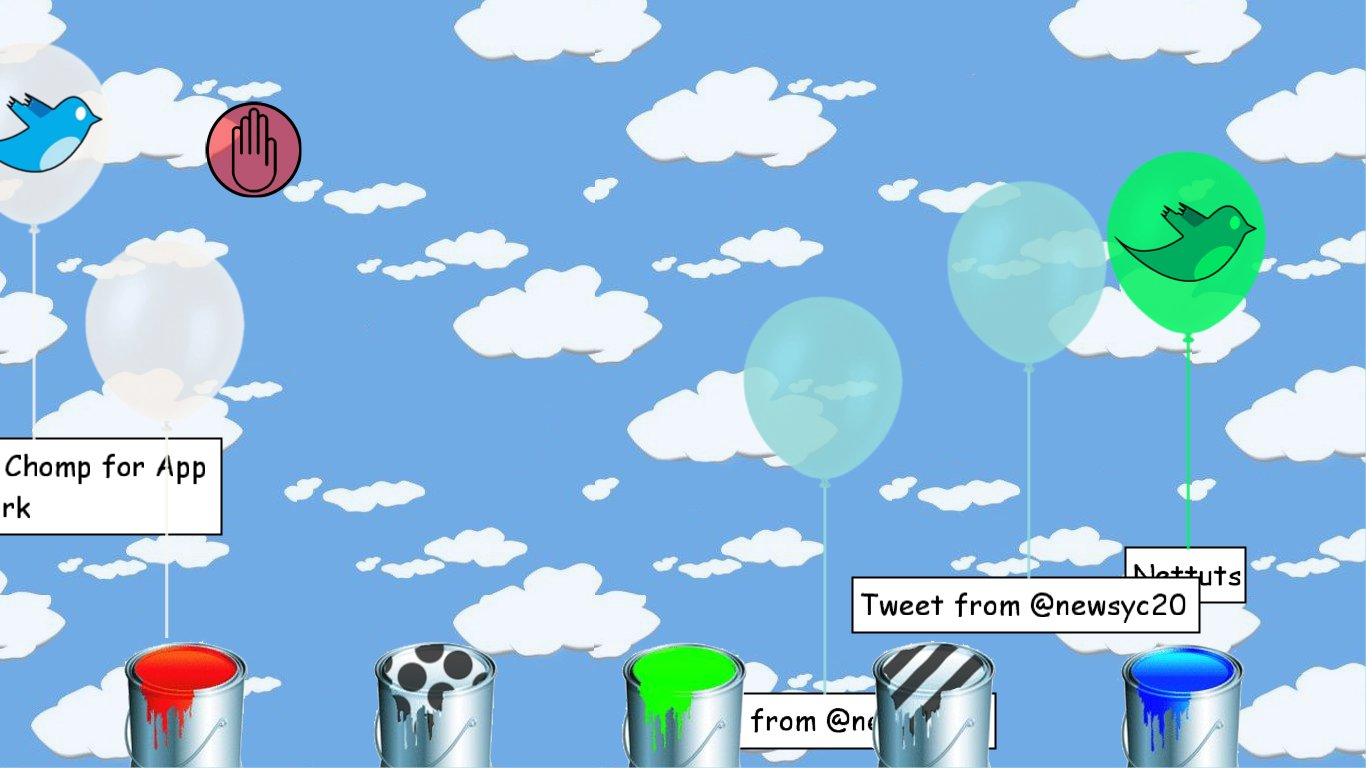
\includegraphics[width=\textwidth]{Diagrams/Client-Log-W6-XNA.jpg}
\par\end{centering}

\caption{Prototype in Week 6 Using XNA Labels}
\end{figure}
\begin{figure}[p]
\begin{centering}
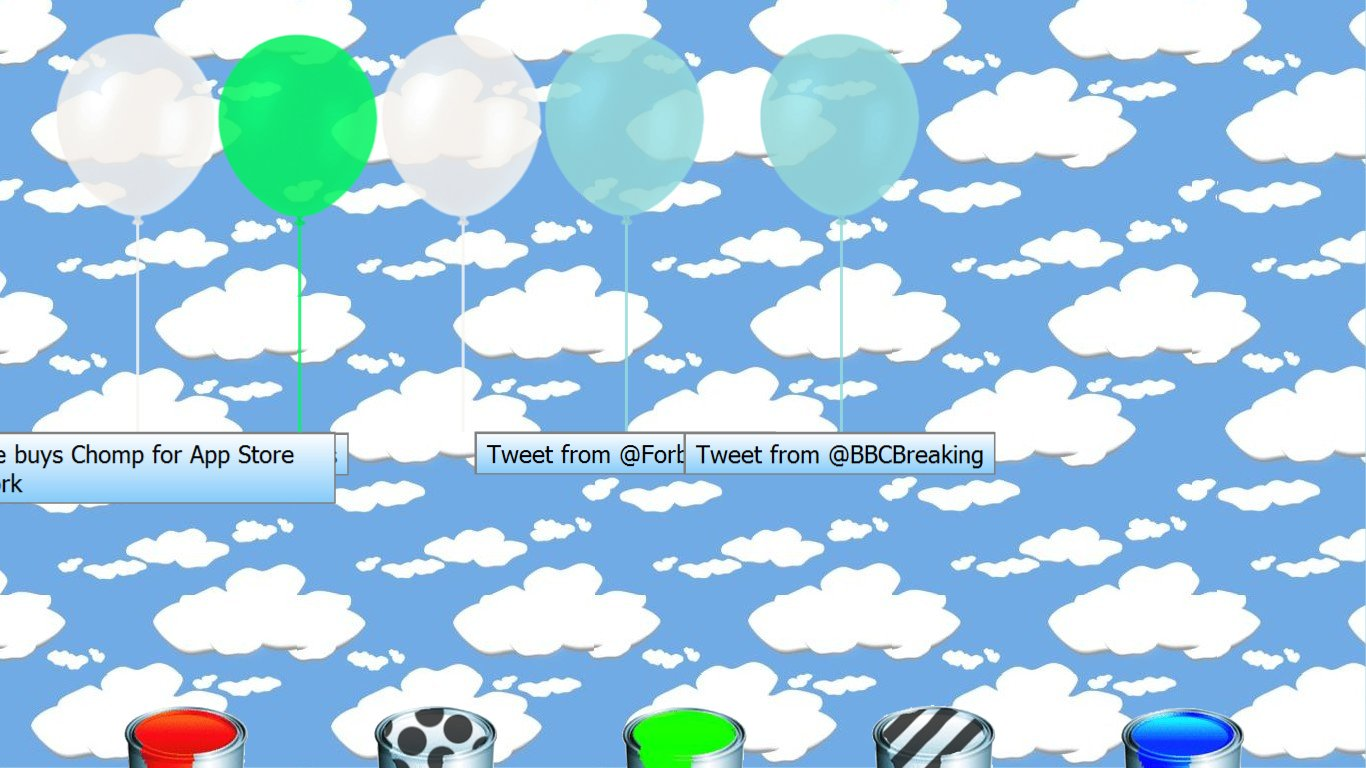
\includegraphics[width=\textwidth]{Diagrams/Client-Log-W6-HTML.jpg}
\par\end{centering}

\caption{Prototype in Week 6 Using HTML Labels}
\end{figure}
Several bug fixes and improvements were implemented for this build. Crashes 
from the previous build were ironed out and fixed; the issue with the user 
being unable to reach the top of the screen was also fixed. Text-wrapping on 
the balloon tags was fixed and the tag boxes made to fit the text once it had
been wrapped to remove any extra white space.

The content box was improved and made to show images and a QR Code which 
encoded the URL of the content article, allowing a user to visit that link with
a mobile device. A timer was added to the content box showing the user how long
until it automatically closed and a large button was placed in the top right of
the screen which the user could use to close the box themselves. An HTML 
version of the content box was also implemented, it was planned to replace the
hard coded versions in the final release. 

Overall the client was very pleased with the improvements made to the system.
Unfortunately it seemed impossible that the Client System could be run on the
target hardware; this demo was shown using a laptop hooked up to the screens
rather than the hardware.

\subsubsection{User Evaluation Build - 27th February}
During the user evaluation some fixes were applied to prevent concurrency 
issues in the HTML renderer when rendering images; other than this the Client 
system's build was unchanged from the previous week.

\subsubsection{User Evaluation Iteration - 13th March}
\begin{figure}[h]
\begin{centering}
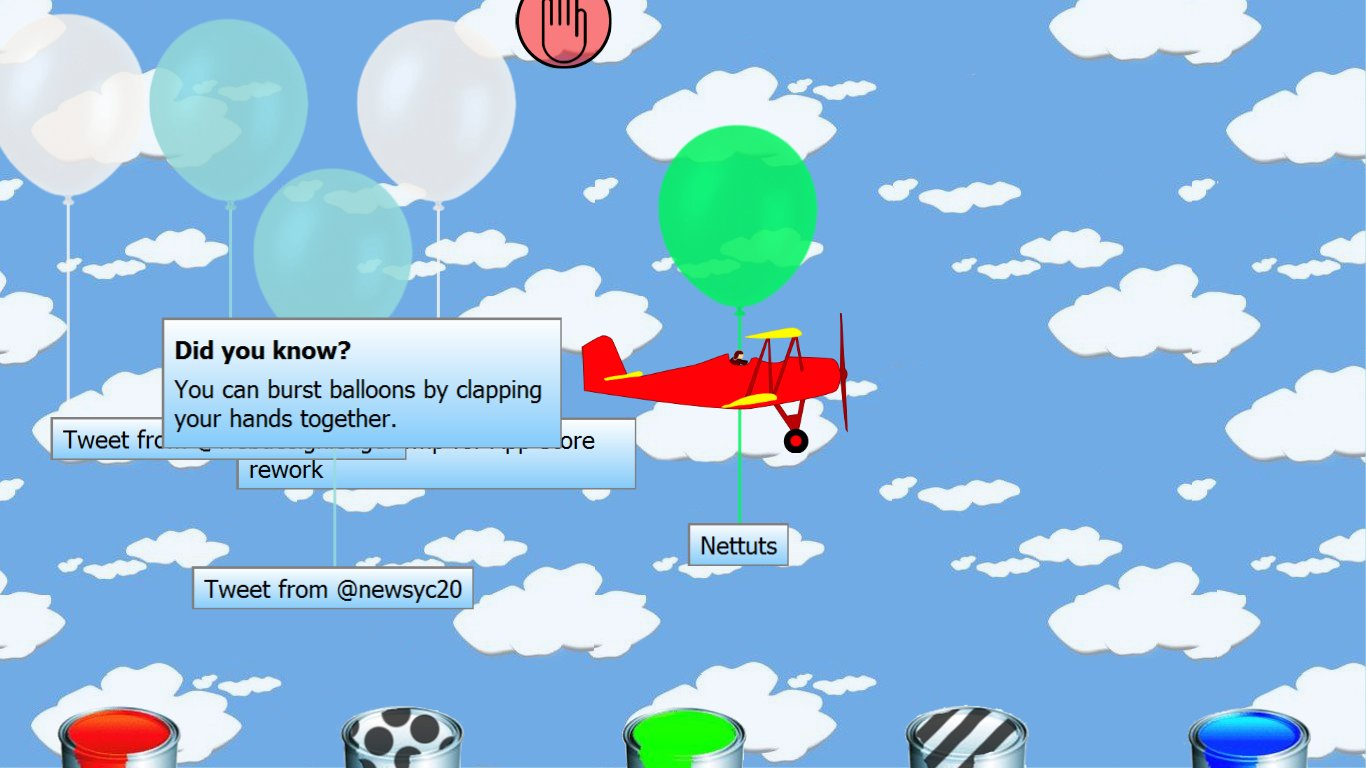
\includegraphics[width=\textwidth]{Diagrams/Client-Log-W10.jpg}
\par\end{centering}

\caption{Final Product}
\end{figure}
From the results of the user evaluation we implemented several fixes to do with
usability --- these included:
\begin{itemize}
\item{Tweaks to the close button for the content box which users found clunky 
to use. We added a black border to it, reduced the activation time from 2.5s to
0.5s and added a second close button in the top-left.}
\item{Paint buckets were too close together; they were spaced out slightly 
further.}
\item{The physical floor was raised slightly whilst moving the buckets down. 
This prevents balloons from being ``stuck'' under the floor.}
\item{Animations were added after a period of inactivity which inform the user
of actions they can take to interact with the system.}
\end{itemize}

\clearpage{}

\subsection{Third-Party Components}
The Client system makes use of several third-party components to reduce the 
amount of development required:

\begin{itemize}
\item{Microsoft XNA Game Studio 4.0}

An environment for quickly creating games which provides several library 
functions such as loading content and drawing to the screen. 
\item{Microsoft Kinect SDK 1.0}

The official SDK providing the ability to interact with the Kinect hardware. 
\item{Farseer Physics 3.3}

A physics library derived from Box2D, a very popular physics library on which
many iPhone and Android games are based. It is used to provide collision 
detection and object interaction between balloons and gives a realistic feel to
balloon movement.
\item{Terra Informatica HTMLayout}

A lightweight HTML renderer used to render the labels and content boxes of 
balloons. This allowed us to provide much richer content than the built-in text
rendering abilities of XNA.
\item{ThoughtWorks QRCode}

A QRCode generation library, used to convert content URLs into a format which 
can be quickly recognised by a user's device.
\end{itemize}


\clearpage{}
\sectionauthor{Kinect Input \& Gestures}{William Reily}
\subsection{Kinect Input}
The Kinect SDK allows us to register for different types of data to get from the device. These are: colour stream, depth stream and skeleton data. We only get the skeleton data since this gives us hand location data. However, this requires the full skeleton to be tracked to just get the hands. This means we can't track a single hand on its own. We could use the depth input and try to find hand locations ourselves, but this is extremely hard for little gain, and it probably wouldn't be as accurate as the skeleton data.
We added the ability to adjust the scaling of the Kinect input into an option in the configuration file. This allowed for adjustment for people of smaller height. We chose to make this a configuration option rather than a hardcoded value because the placement of the Kinect in relation to the user can affect the user's ability to reach parts of the screen. We also scale the x and y axis input separately since people can usually reach from left to right easier than reaching vertically.

One disadvantage to this scaling is it adversely affects the accuracy of the Kinect. The Kinect sensor does not track the user perfectly, especially the extremities such as the hands. As such the position of the person's hand is constantly in flux, even when the real hand is stationary. Increasing the scaling factor of the Kinect amplifies this inaccuracy. This can cause the hand to excessively jitter, and makes clapping much more difficult. As such, the values should be left to as low as is still usable.
We did find that the angle of the Kinect and distance from the Kinect affected the difference in height greatly. Having a direct angle at mid-distance provided the most consistent usability between users.

There are some hardware limitations of the Kinect however. For example, users in wheelchairs may have some difficulty in using the Kinect. Because we use skeleton tracking to find hand positions, if the Kinect has issues tracking the full user, then the hands can't be displayed. The Kinect will often interpret a wheelchair or crutches as legs, but this may not be a significant issue for us, since we only require the hands be accurately tracked. However, we did find that large jackets interfered with the hand positions.
We also found the minimum hardware on the connected machine to run the Kinect was surprisingly high. It would seem the Kinect can be quite a CPU hog.

\clearpage{}
\subsection{Developer Documentation}
The Kinect Controller Input class (see table \ref{KinectInputRef}) is the implementation of the IInputManager interface for the Kinect device. It registers to the Kinect that it wants to receive skeleton data, which it then uses to generate hand objects. The Kinect sends us data by means of a callback method, so we have to use a lock to ensure GetHandPositions doesn't happen during the middle of an update.

\begin{table}[h]
\begin{tabular}{|>{\raggedright}p{5cm}|>{\raggedright}p{3.6cm}|>{\raggedright}p{7cm}|}
\hline 
\multicolumn{3}{|c|}{KinectControllerInput}\tabularnewline
\hline 
Initialize & Screen Size & Implementation from IInputManager. This sets the scaling variables
and attempts to connect to the Kinect.\tabularnewline
\hline 
GetHandPositions & Returns Hand{[}{]} & Implementation from IInputManager. See description in IInputManager.\tabularnewline
\hline 
convertRawHandToScreen & SkeletonPoint, Returns Vector2 & Converts a raw skeleton point from the Kinect skeleton data to a screen
coordinate. This method is just a wrapper around the Vector2 method
below.\tabularnewline
\hline 
convertRawHandToScreen & Vector2,\newline Returns Vector2 & Converts a raw point from the Kinect to screen coordinates. It applies
a scaling factor in each axis and the transforms it from the raw coordinate
space to screen coordinate space (defined in Initialize).\tabularnewline
\hline 
SkeletonsReady & Sender Object,\newline Event Args & This is a callback function that is assigned when the Initialize method
is called. It gets called once for each frame the Kinect calculates.
It uses the skeleton data to generate hand data.\tabularnewline
\hline 
\end{tabular}

\caption{\emph{KinectControllerInput} reference}

\label{KinectInputRef}
\end{table}

\clearpage{}
\subsection{Gestures}

We had originally designed the system to use multiple gestures to manipulate and navigate it; however through advice and some minor experimentation, we chose not to do this since recognising gestures is very difficult. The Kinect has no native support for recognising gestures, so it is left to the programmer to implement these. We refined the application to use only a clapping gesture, and just use the hand positions for the rest.

We originally implemented the clap as checking if two hands are touching the same balloon, however this caused too many false positives. Users would burst balloons when they only meant to knock them, often by rapidly moving their arms around.
We then improved this method by adding additional conditions to trigger a clap. These are:

\begin{itemize}
\item{The hands must be moving towards the balloons (with an angle of tolerance).}
\item{The hands must be moving towards to each other (again, with an angle of tolerance).}
\item{Both hands must be moving above a certain speed.}
\end{itemize}

This did help to remove the false positives; however it did make it harder to actually burst a balloon, to the point users were having difficulty popping a balloon. We added each tolerance as an option in the configuration file, so this can be adjusted easily to a value that feels natural. We found through testing that setting the tolerances to be very generous (high angles, low speeds) was best, as an occasional accidental balloon burst was better than an extremely difficult time popping a balloon.

Both of these methods use a reactive approach, only checking the conditions at the moment of impact between the hand and the balloon, however the Kinect sensor can adds extra jitter and inaccuracies to the data (as noted in Kinect section). If a jitter occurs just at the moment of impact (which it frequently does), then it will not register a clap (as the hands are not moving quite towards each other/the balloon in that frame), which is mainly why setting low tolerances helped.

A better method would be to continuously track the hands and detect when a clap is happening, as this reduces the influence of random jitter in the data stream. Alternatively, if we calculated the velocity of the hand objects ourselves as a normalised sum of the n previous frames, this would help reduce noise in the data.
 


\clearpage{}
\sectionauthor{Server Design}{Brieuc Roblin \& Pierre-Andr\'{e} Saulais}
%In this section we describe what the Balloon Server does and how it fits in the
project. 

\subsection{Specifications}

The goal of the Balloon Server is to make users believe that, no matter how
many screens are used for display, there is only one Balloon application. One
way to achieve this is to make the screens look `connected'. That is, after
pushing a balloon through the left edge of a screen, the balloon should
reappear at the right edge of another screen. Another way is to enforce that a
balloon is shown only on one screen at any given time.

We want users to believe that the balloon that appeared in one screen is the
same balloon that disappeared in the other screen. Since the appearance of
balloons is customisable (the colour and texture can be changed by the user),
believing they are the same is easier if customisations are kept when
transferring the balloon from one screen to another. In addition, it is more
believable if balloons keep their speed and direction when moving across 
screens.

The server is responsible for notifying the client when balloons should appear
on its screen and how (e.g. what type of balloon, caption text, content
to show when popping the balloon). The server does not create the data needed to
display balloons itself. This task is the responsibility of the Web Feed. In
order to have balloons to provide to the client, the server has to regularly
retrieve the information needed to create these balloons from the feed.

Something to keep in mind is that the content of this feed changes with time
(new items are added from the Twitter aggregator and user-submitted 
content) but we want to keep the number of balloons on a screen at a
reasonable level. This is why the server has to decide which balloons should be
kept and which should be discarded when new items are retrieved from the feed.
We have decided to discard all balloons without a matching feed item.

An additional requirement is that the number of screens connected to the server
is not fixed and can change over the lifetime of the server execution. 
Connecting and disconnecting screens from the server can be done at
any time and does not interfere with the processing of balloons. For example, 
when a screen is added the server requests more items from the feed. These new
items are used to create new balloons to populate the new, empty screen. When 
disconnecting a screen, its balloons are transferred to the remaining screens.

Late in the project, we decided to introduce on-screen `tips' to help new users
interact with our application. This was materialised as a plane carrying a label
showing the tip banner behind it. The server is responsible for deciding when 
such planes are shown, transferring them between screens and deciding when they
have to disappear. Indeed we felt that always having a plane on a screen could
be annoying for the users, especially since planes can collide with balloons 
and push them away when users might be interacting with them.

\clearpage{}
\subsection{Design}

As the server is a self-contained part of the project, we have decided to 
develop it as a separate program. This allowed us to have clear interfaces 
between the server and other parts of the project and made it easier for
multiple people to work on different parts of the project at the same time.
Most of the communication happens between the client and the server, which 
meant that writing the server in the same language than the client (C\#) let us 
share much code between the two and let the client team focus on client issues 
and not network issues.

The server communicates with the feed through the standard HTTP protocol 
(using JSON to format feed data) and with the Balloon Client through a custom 
protocol that is used over TCP/IP sockets. The former choice was decided by the 
Web team and motivated by ease of use and reuse of existing libraries. As far 
as we are aware there is no existing protocol that lets coordinating content
balloons over different screens, therefore we had to create our own. Using 
sockets instead of higher-level communication frameworks was chosen 
to make debugging easier by writing explicit code at the expense of writing 
more code.

\subsubsection{Messaging}

There is in general two ways to communicate between two applications: messaging 
and Remote Procedure Call. We have chosen the former as we have some experience 
with it. We also believe it is easier to design a networked application when 
requests and responses are represented and passed around explicitly (e.g. as 
messages). In particular, the messaging approach makes it easier (and obvious) 
in which thread a message is processed. This is especially important in the 
client where drawing the game must be done in a special thread.

With a messaging approach, the interface between client and server is defined by 
a set of messages that can be sent by one or the other or both (see figures 
\ref{ServerMessages}, \ref{ClientMessages} and \vref{CommonMessages}). The most
important messages are NewBalloon/PopObject (they control balloons appearing/
disappearing on the screen) and ChangeScreen (controls balloons moving between
screens).

\begin{table}
\begin{tabular}{|>{\raggedright}p{4.3cm}|>{\raggedright}p{2.8cm}|>{\raggedright}p{8.7cm}|}
\hline 
Message Name & Parameters & Description\tabularnewline
\hline 
NewBalloon
& Balloon ID 
\newline Direction
\newline Position (Y)
\newline Velocity (X, Y)
& A new balloon should appear on the screen at the given screen height (Y position),
with the given direction and on the side of the screen given by the direction.
\tabularnewline
\hline 
NewPlane
& Plane ID 
\newline Plane type
\newline Direction
\newline Position (Y)
\newline Velocity (X, Y)
\newline Time
& A new plane should appear on the screen at the given screen height (Y position),
with the given direction, on the side of the screen given by the direction, with
a message given by its type and with the specified initial animation time.
\tabularnewline
\hline 
BalloonContentUpdate
& Balloon ID 
\newline Balloon type
\newline Label
\newline Content
\newline URL
\newline Image URL
& Indicates that the content of the specified balloon (caption label, content
text to display when the balloon is popped, URL to the article, URL to the image) 
has been changed. 
\tabularnewline
\hline 
\end{tabular}

\caption{Messages sent by the server}

\label{ServerMessages}
\end{table}

\begin{table}
\begin{tabular}{|>{\raggedright}p{4.3cm}|>{\raggedright}p{2.8cm}|>{\raggedright}p{8.7cm}|}
\hline 
Message Name & Parameters & Description\tabularnewline
\hline 
ChangeScreen
& Balloon ID 
\newline Direction
\newline Position (Y)
\newline Velocity (X, Y)
\newline Time
& The given balloon or plane moved off the screen at the given screen height (Y position),
with the given direction and on the side of the screen given by the direction. For planes,
the time value is the current animation time.
\tabularnewline
\hline 
GetBalloonContent
& Balloon ID
& Request that the content of the specified balloon be sent to the client.
\tabularnewline
\hline 
GetBalloonState
& Balloon ID
& Request that the state of the specified balloon be sent to the client.
\tabularnewline
\hline 
\end{tabular}

\caption{Messages sent by the client}

\label{ClientMessages}
\end{table}

\begin{table}
\begin{tabular}{|>{\raggedright}p{4.3cm}|>{\raggedright}p{2.8cm}|>{\raggedright}p{8.7cm}|}
\hline 
Message Name & Parameters & Description\tabularnewline
\hline 
PopObject
& Balloon ID or plane ID
& When sent by the client, indicates that the user popped the specified balloon.
When sent by the server, indicates that the specified balloon or plane has been 
removed from the screen (after updating the feed).
\tabularnewline
\hline 
BalloonStateUpdate
& Balloon ID
\newline Overlay type
\newline Background colour
\newline Number of votes
& Indicates that the state of the given balloon (overlay texture, background colour
and number of votes) has been changed. This can be sent by the server when the 
number of votes changes or by the client when the user changes a balloon's 
decoration with paint buckets.
\tabularnewline
\hline 
\end{tabular}

\caption{Messages sent by both client and server}

\label{CommonMessages}
\end{table}

One important aspect of this communication is that it is asynchronous. This 
means that messages are sent as a kind of notification to the recipient. The 
sender does not wait for a `return receipt' from the recipient before resuming 
its activity. Indeed in general it does not need to know when the message has
arrived. The only exception comes with the GetBalloonContent/GetBalloonState 
messages which are answered by BalloonContentUpdte/BalloonStateUpdate messages.
Howerver, the latter messages can be also sent spontaneously (e.g. when the user 
changes a balloon's decoration using the paint buckets). Messages are handled 
the same no matter if they are spontaneous or a response from another message.

\begin{table}[h]
\begin{tabular}{|p{4.4cm}|p{3.6cm}|p{7.6cm}|}
\hline
\multicolumn{3}{|c|}{ScreenConnection} \\ \hline
\emph{Constructor} & Message Queue & Creates a new connection object with no established connection. 
Received messages will be added to the queue. \\ \hline

\emph{Constructor} & Message Queue, \newline Socket & Creates a new connection 
object with an established socket connection. Received messages will be added to the queue. \\ \hline

Connect & IP Address, \newline Port & Try to establish a socket connection to the Server at the given address and port. \\ \hline

StartReceivingMessages & & Start receiving messages from an established connection. \\ \hline

SendMessages & Message & Sends a message on an established connection. \\ \hline

\end{tabular}

\caption{\emph{ScreenConnection} reference}

\label{ScreenConnRef}
\end{table}

Sockets can only send and receive bytes. This is why there must be a way to
transform message objects from and to bytes, in order to transmit them over the
networks between the screens and server. This process is called serialisation. 
During this project we have implemented two serialisation formats. The first is
a text-based format based on JSON and was used for the first prototypes of our 
project. Text-based formats are usually very flexible and easy to debug; on
the other hand they are quite slow to manipulate. This is why a second, binary
serialiser was written after the first prototypes were successful.


\subsubsection{Architecture}

The main reason from shying away from communication frameworks and libraries was
to be able to easily change the architecture (in particular, threading) of the 
server if the need arose. Possible issues that come with a bad threading design 
include non-intuitive behaviour; subtle, difficult-to-reproduce bugs and low 
performance. This is why it was important to have a good architecture to avoid 
these issues as much as possible. We had to change it multiple times during the 
course of this project when we ran into some of these issues.

\begin{figure}
\begin{centering}
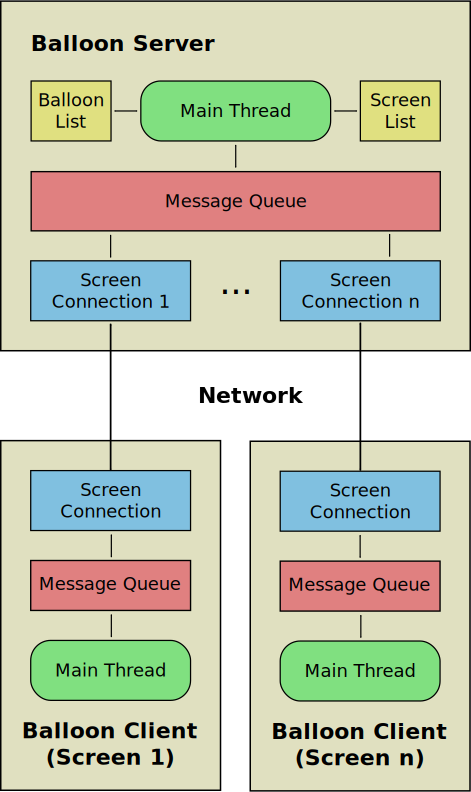
\includegraphics[scale=0.95]{Diagrams/messaging}
\par\end{centering}

\caption{Messaging and Threading Architecture}
\label{Messaging-Arch}
\end{figure}

The final architecture (see figure \vref{Messaging-Arch}) tries to minimise the
use of threads. In particular, in both client and server, as much processing as
possible is done in a single thread (`Main thread' for the server, `GUI thread'
for the client). However, messages received over the network
can arrive in any thread (this is because we are using asynchronous I/O). To 
keep all processing on the main thread, messages are placed in a thread-safe
message queue and then removed in order by the main thread when it is ready. 

This design pattern (thread with a message/event loop) is used throughout the
application. In the client, the GUI thread has a message queue which it empties
during the `Update' phase. In the server, both the main thread and feed reader 
thread have a message queue; they communicate by placing messages in each other's
queue. This approach limits the need for synchronisation between threads and 
thus avoids associated pitfalls.

The reason we have a separate thread for the feed reader is that pulling the 
feed can take a long time (several seconds). If this was done on the main 
thread, during this time the server would be blocked (e.g. balloons would not 
reappear on another screen after moving out of one screen) which we wanted to 
avoid. With this approach, the feed reader thread is blocked when updating the
feed while the main thread can continue processing. When the update is done, the
new feed items are placed in the message queue and processed by the main thread.
Similarly in the client, long-running operations such as downloading images and 
rendering HTML pages are done on a background thread and the result is used in 
the GUI thread.

\subsection{Persistence}

By persistence, we mean saving the balloon data manipulated by the server between 
executions. Persisting balloon data means that when shutting down the 
server and then starting it again this data would be preserved. Since it 
originates from the feed and can be re-queried at will, we have chosen not to
have any persistence for balloon data. However, some data is persisted across 
execution as we will see in the next section about configuration.

Even though we have made this choice, this does not mean persistence could not 
be implemented for this project in the future. The serialisation and message 
classes we wrote to support communication between client and server could be 
reused fairly easily to this end (e.g. serialising messages to a buffer and 
then writing this buffer to a file).

\subsection{Configuration}

This part of the application was at the beginning only intended to be used by 
the server but was later extended to the client as well. It puts together many 
variables that change the behaviour of the application (e.g. how many balloons 
to show on each screen, which URL to query the feed from, how often it  
should be queried, etc). The value of these variables can be written to or read 
from a file by the application. We have chosen the JSON format for such files, 
which is easily manipulated with a text editor. When the server (or client) is 
started and this file does not exist, a file containing default values for the 
variables is created.



\clearpage{}
\sectionauthor{Web Feed Design}{Christopher Wyllie}
\subsection{Technologies}

Construction of the web components of this project was undertaken with the following technologies:

\begin{itemize}
	\item Apache 2
	\item PHP 5
	\item MySQL 5
\end{itemize}

The main reason behind this is that these technologies are available inside the University network, and they are widely understood by most of the development team.

In order to facilitate the rapid and robust development necessary, the following libraries and frameworks were used:

\begin{itemize}
	\item Code Igniter PHP Framework
	\item JQuery Mobile toolkit
	\item tmhOAuth PHP Twitter library
\end{itemize}

Choice of each library was based on ease of use, and how much value they can add to the project by providing ready to use components for common tasks such as handling file uploads.

\subsection{Web System Overview}

\subsubsection{Content Feed}

The balloon application relies upon content delivered by a web-accessible 'feed'. This feed is designed to aggregate various information sources, and provide a single authoritative reference for content to be displayed.

Currently the feed provides information from the following sources:

\begin{itemize}
	\item User generated content
	\item Twitter aggregation account
\end{itemize}

In addition to these content sources, the feed introduces blank balloons, and is responsible for selecting an appropriate number of each content type based on the total number of items requested. The following section will cover each content type in more detail.

\subsubsection{Content Proxy}
To facilitate a more engaging user interaction with content, a proxy is used when a user visits the link for any piece of content. This proxy allows votes for user generated content to be recorded, and would allow future extensions to be made to the way content is delivered to the user.

\subsection{Content Types}

\subsubsection{User Generated Content}
By using the content submission portal, it is possible for MACS students to submit their own content to be shown on the screens. Content submitted by users is considered a priority over the other content types, but because it is expected to be posted less frequently, it may not feature heavily in the feed's content.

It is possible for users to vote on this content type, with the number of votes influencing how likely the content is to be displayed.

This content type will be selected with the most recent submissions first, up to the limit requested.

\subsubsection{Top-rated User Generated Content}
If an item submitted by a user receives lots of positive votes, it will assume the pseudo content type of 'top-rated'. Top-rated content will always feature in the feed, and be chosen at random from all top-rated items.

This content type is distinct from the most recent items, and items selected for this type will not be considered for the most recent item selection.

If the content item receives negative votes in this state, it is possible for it to lose its top-rated status, and it will become available for selection again to the most recent items.

\subsubsection{Twitter}
In order to create a dynamic, relevant information feed, a Twitter account Macs\_Aggregator has been used to provide news items. This account follows a variety of industry news outlets and accounts of interest to students in the Edinburgh area.

\subsubsection{Blank Balloons}
The feed introduces balloons that are deliberately left blank to allow users to customise their appearance.

\subsection{Feed Construction}

\subsubsection{Content Balancing}
To ensure that there will always be enough content available for every connected screen, and that no one content type will unintentionally dominate other content types, the feed's items are balanced according to a configurable ratio.

The file \texttt{application/config/feed.php} defines the content types and the values of the ratio in the \texttt{FeedContentTypes} class. It also gives the thresholds for votes which will make a balloon top-rated, or prevent a balloon from showing up again.

Constants from the \texttt{FeedContentTypes} class are used throughout the application code to aid readability and reduce the likelihood of errors.

\subsubsection{Controller}
The file \texttt{application/controllers/api.php} implements a factory to generate feed items, and the public endpoint to access these items from.

\texttt{Api::getFeed} will use the ratio defined in the feed config and the number of items requested to work out how many of each content type to include. In the case that the total number of items requested cannot be fulfilled by the available user generated content, the feed will include extra tweets to make up the difference.

The public endpoint will return a JSON encoded feed of items in a standard format, regardless of initial content type.

\subsection{Content Proxy}
Every link presented in a QR code will pass through the content proxy page, which decides what to do based on the content type. The purpose is currently three-fold:

\begin{enumerate}
	\item Allow users to rate user generated content by voting on it
	\item Ensure that the URLs presented for the QR codes are at most 86 characters
	\item Provide an easy mechanism to adjust control flow in the future
\end{enumerate}

The \texttt{Content} and \texttt{Url} controllers are responsible for handling this process. It is a two-step process with the \texttt{Url} controller handling short URL redirection, and the \texttt{Content} controller implementing the intermediate voting interfaces.

\subsubsection{Content Ratings}
When a user scans the QR code for user generated content items, they will be presented with a page that allows them to vote the content up and down.

The \texttt{Content} controller defined in \texttt{application/controllers/content.php} manipulates the \texttt{Content\_model} to facilitate this voting.

\texttt{Content::visit} will look up the content item by ID and present the voting interface to the user. This interface is built using the JQuery Mobile toolkit\footnote{http://jquerymobile.com}. This toolkit allowed a cross-platform interface with standard components to be constructed with ease.

On the voting page, the user is presented with three links. One link takes them to the content, and the other two links correspond to the \texttt{Content::up} and \texttt{Content::down} methods which cost a vote and then redirect to the content link.

\subsubsection{URL Shortening}
Due to the size limitation of 86 characters in the QR code version chosen, it is necessary to shorten all URLs passed in the feed. Doing this ensures that every URL will be less than the 86 character limit.

To facilitate this, a simple database table is used to store URLs with an integer ID. The model \texttt{Url\_map} is then used to shorten and expand URLs based on this integer ID.

Short URLs take the form of \texttt{baseURL + shortID}, and it is this shortID that will be used to retrieve the original URL.

When using the model to shorten a URL, it is necessary to configure it with the base URL you want the shortened URL to point to. This is accomplished with the \texttt{Url\_map::set\_base\_url} method. Once configured, the \texttt{shorten} method will return a short URL relative to the base URL set.

In order to resolve a short URL to the original URL, the \texttt{Url\_map::unshorten} method is used. This method expects to be given the ID it returned as the last part of the short URL.

To achieve the maximum possible compression, the integer ID stored in the database table is base-62 encoded by the \texttt{shorten} function, and base-62 decoded by the \texttt{unshorten} method.

The \texttt{Url} controller implements a method to redirect from the short URL to the original URL.

\subsubsection{Future Possibilities}
By providing a central point through which all traffic must pass, there is the potential to collect statistics about what is being visited the most frequently, and also to present additional user interfaces upon scanning of a QR code.

\subsection{Future Work}

\subsubsection{Feed Generation}
It would be good to refactor the current feed generation method to use a slightly more abstract factory pattern. The initial groundwork is in place with the \texttt{BlankBalloonFactory} class, but this could be abstracted further.

Ideally each content type would have its own factory class which all extend a common parent class, or implement a \texttt{BalloonFactory} interface.

This would allow the code in the \texttt{Api} controller to be simplified, and increase its modularity allowing further content types to be added with ease.

\subsubsection{Usage Metrics}
It would be possible to use the content proxy as mentioned to gather statistics on usage. By gathering information on what types of content users tend to visit, the feed's content ratios could be adjusted, or even evolve dynamically for given times of day dependent on previous usage patterns.

\subsubsection{Mobile Content Submission UI}
Balloons could be introduced to the feed that would link to a mobile optimised content submission portal. This interface could be built with the JQuery Mobile toolkit and integrate with the existing controller and model setups.

\subsubsection{Saving of Customised Balloons}
It would be possible for the clients to provide a link to the web where a user could save an image of their customised balloon.

\subsubsection{Additional Content Types}
It would be possible to introduce new content types to the feed, such as items from RSS feeds, or direct messages sent to the Macs\_Aggregator Twitter account.


\clearpage{}
\section*{Conclusion}
\addcontentsline{toc}{section}{Conclusion}
\markboth{Conclusion}{}


\clearpage{}
\appendix
\thispagestyle{empty}
\vspace*{\fill}
\begin{flushright}
\textsf{\textbf{\huge Appendices}}\vspace*{\fill}
\par\end{flushright}
\vspace*{\fill}
\pagebreak{}

\section{Appendix: Configuration File}

\end{document}
